% Options for packages loaded elsewhere
\PassOptionsToPackage{unicode}{hyperref}
\PassOptionsToPackage{hyphens}{url}
%
\documentclass[
  man, donotrepeattitle,floatsintext]{apa6}
\usepackage{amsmath,amssymb}
\usepackage{lmodern}
\usepackage{iftex}
\ifPDFTeX
  \usepackage[T1]{fontenc}
  \usepackage[utf8]{inputenc}
  \usepackage{textcomp} % provide euro and other symbols
\else % if luatex or xetex
  \usepackage{unicode-math}
  \defaultfontfeatures{Scale=MatchLowercase}
  \defaultfontfeatures[\rmfamily]{Ligatures=TeX,Scale=1}
\fi
% Use upquote if available, for straight quotes in verbatim environments
\IfFileExists{upquote.sty}{\usepackage{upquote}}{}
\IfFileExists{microtype.sty}{% use microtype if available
  \usepackage[]{microtype}
  \UseMicrotypeSet[protrusion]{basicmath} % disable protrusion for tt fonts
}{}
\makeatletter
\@ifundefined{KOMAClassName}{% if non-KOMA class
  \IfFileExists{parskip.sty}{%
    \usepackage{parskip}
  }{% else
    \setlength{\parindent}{0pt}
    \setlength{\parskip}{6pt plus 2pt minus 1pt}}
}{% if KOMA class
  \KOMAoptions{parskip=half}}
\makeatother
\usepackage{xcolor}
\usepackage{graphicx}
\makeatletter
\def\maxwidth{\ifdim\Gin@nat@width>\linewidth\linewidth\else\Gin@nat@width\fi}
\def\maxheight{\ifdim\Gin@nat@height>\textheight\textheight\else\Gin@nat@height\fi}
\makeatother
% Scale images if necessary, so that they will not overflow the page
% margins by default, and it is still possible to overwrite the defaults
% using explicit options in \includegraphics[width, height, ...]{}
\setkeys{Gin}{width=\maxwidth,height=\maxheight,keepaspectratio}
% Set default figure placement to htbp
\makeatletter
\def\fps@figure{htbp}
\makeatother
\setlength{\emergencystretch}{3em} % prevent overfull lines
\providecommand{\tightlist}{%
  \setlength{\itemsep}{0pt}\setlength{\parskip}{0pt}}
\setcounter{secnumdepth}{-\maxdimen} % remove section numbering
% Make \paragraph and \subparagraph free-standing
\ifx\paragraph\undefined\else
  \let\oldparagraph\paragraph
  \renewcommand{\paragraph}[1]{\oldparagraph{#1}\mbox{}}
\fi
\ifx\subparagraph\undefined\else
  \let\oldsubparagraph\subparagraph
  \renewcommand{\subparagraph}[1]{\oldsubparagraph{#1}\mbox{}}
\fi
\newlength{\cslhangindent}
\setlength{\cslhangindent}{1.5em}
\newlength{\csllabelwidth}
\setlength{\csllabelwidth}{3em}
\newlength{\cslentryspacingunit} % times entry-spacing
\setlength{\cslentryspacingunit}{\parskip}
\newenvironment{CSLReferences}[2] % #1 hanging-ident, #2 entry spacing
 {% don't indent paragraphs
  \setlength{\parindent}{0pt}
  % turn on hanging indent if param 1 is 1
  \ifodd #1
  \let\oldpar\par
  \def\par{\hangindent=\cslhangindent\oldpar}
  \fi
  % set entry spacing
  \setlength{\parskip}{#2\cslentryspacingunit}
 }%
 {}
\usepackage{calc}
\newcommand{\CSLBlock}[1]{#1\hfill\break}
\newcommand{\CSLLeftMargin}[1]{\parbox[t]{\csllabelwidth}{#1}}
\newcommand{\CSLRightInline}[1]{\parbox[t]{\linewidth - \csllabelwidth}{#1}\break}
\newcommand{\CSLIndent}[1]{\hspace{\cslhangindent}#1}
\ifLuaTeX
\usepackage[bidi=basic]{babel}
\else
\usepackage[bidi=default]{babel}
\fi
\babelprovide[main,import]{english}
% get rid of language-specific shorthands (see #6817):
\let\LanguageShortHands\languageshorthands
\def\languageshorthands#1{}
% Manuscript styling
\usepackage{upgreek}
\captionsetup{font=singlespacing,justification=justified}

% Table formatting
\usepackage{longtable}
\usepackage{lscape}
% \usepackage[counterclockwise]{rotating}   % Landscape page setup for large tables
\usepackage{multirow}		% Table styling
\usepackage{tabularx}		% Control Column width
\usepackage[flushleft]{threeparttable}	% Allows for three part tables with a specified notes section
\usepackage{threeparttablex}            % Lets threeparttable work with longtable

% Create new environments so endfloat can handle them
% \newenvironment{ltable}
%   {\begin{landscape}\centering\begin{threeparttable}}
%   {\end{threeparttable}\end{landscape}}
\newenvironment{lltable}{\begin{landscape}\centering\begin{ThreePartTable}}{\end{ThreePartTable}\end{landscape}}

% Enables adjusting longtable caption width to table width
% Solution found at http://golatex.de/longtable-mit-caption-so-breit-wie-die-tabelle-t15767.html
\makeatletter
\newcommand\LastLTentrywidth{1em}
\newlength\longtablewidth
\setlength{\longtablewidth}{1in}
\newcommand{\getlongtablewidth}{\begingroup \ifcsname LT@\roman{LT@tables}\endcsname \global\longtablewidth=0pt \renewcommand{\LT@entry}[2]{\global\advance\longtablewidth by ##2\relax\gdef\LastLTentrywidth{##2}}\@nameuse{LT@\roman{LT@tables}} \fi \endgroup}

% \setlength{\parindent}{0.5in}
% \setlength{\parskip}{0pt plus 0pt minus 0pt}

% Overwrite redefinition of paragraph and subparagraph by the default LaTeX template
% See https://github.com/crsh/papaja/issues/292
\makeatletter
\renewcommand{\paragraph}{\@startsection{paragraph}{4}{\parindent}%
  {0\baselineskip \@plus 0.2ex \@minus 0.2ex}%
  {-1em}%
  {\normalfont\normalsize\bfseries\itshape\typesectitle}}

\renewcommand{\subparagraph}[1]{\@startsection{subparagraph}{5}{1em}%
  {0\baselineskip \@plus 0.2ex \@minus 0.2ex}%
  {-\z@\relax}%
  {\normalfont\normalsize\itshape\hspace{\parindent}{#1}\textit{\addperi}}{\relax}}
\makeatother

% \usepackage{etoolbox}
\makeatletter
\patchcmd{\HyOrg@maketitle}
  {\section{\normalfont\normalsize\abstractname}}
  {\section*{\normalfont\normalsize\abstractname}}
  {}{\typeout{Failed to patch abstract.}}
\patchcmd{\HyOrg@maketitle}
  {\section{\protect\normalfont{\@title}}}
  {\section*{\protect\normalfont{\@title}}}
  {}{\typeout{Failed to patch title.}}
\makeatother

\usepackage{xpatch}
\makeatletter
\xapptocmd\appendix
  {\xapptocmd\section
    {\addcontentsline{toc}{section}{\appendixname\ifoneappendix\else~\theappendix\fi\\: #1}}
    {}{\InnerPatchFailed}%
  }
{}{\PatchFailed}
\keywords{optimality, moral judgment, theory of mind, lay decision theory\newline\indent Word count: 11,495}
\usepackage{csquotes}
\ifLuaTeX
  \usepackage{selnolig}  % disable illegal ligatures
\fi
\IfFileExists{bookmark.sty}{\usepackage{bookmark}}{\usepackage{hyperref}}
\IfFileExists{xurl.sty}{\usepackage{xurl}}{} % add URL line breaks if available
\urlstyle{same} % disable monospaced font for URLs
\hypersetup{
  pdftitle={Holding Experts to Excessive Epistemic Standards},
  pdfauthor={Samuel H. Borislow1 \& Geoffrey P. Goodwin2},
  pdflang={en-EN},
  pdfkeywords={optimality, moral judgment, theory of mind, lay decision theory},
  hidelinks,
  pdfcreator={LaTeX via pandoc}}

\title{Holding Experts to Excessive Epistemic Standards}
\author{Samuel H. Borislow\textsuperscript{1} \& Geoffrey P. Goodwin\textsuperscript{2}}
\date{}


\shorttitle{Holding Experts to Excessive Standards}

\authornote{

The authors made the following contributions. Samuel H. Borislow: Conceptualization, Writing - Original Draft Preparation, Writing - Review \& Editing; Geoffrey P. Goodwin: Writing - Review \& Editing, Supervision.

Correspondence concerning this article should be addressed to Samuel H. Borislow, 5807 S Woodlawn Ave, Chicago, IL 60637. E-mail: \href{mailto:sbori@chicagobooth.edu}{\nolinkurl{sbori@chicagobooth.edu}}

}

\affiliation{\vspace{0.5cm}\textsuperscript{1} University of Chicago\\\textsuperscript{2} University of Pennsylvania}

\abstract{%
De Freitas and Johnson (2018) found that people are blamed for making suboptimal decisions, even under circumstances in which an optimal decision cannot reasonably be expected (De Freitas \& Johnson, 2018). They termed this phenomenon ``optimality bias,'' and stated that it depended only on a reference to the relevant agents' choices, making no reference to their mental states. More precisely, they stated that suboptimal decisions are seen as more difficult to explain and are, therefore, also perceived to be more deserving of blame. However, what if the cause of this bias is instead an overassessment of the decision makers' abilities (thus, making reference to their mental states)? In a series of three studies, we examined whether thinking that an agent ``should have known better'' predicts blame judgments better than thinking an explanation was needed for their suboptimal behavior, as well as whether this effect is only found when judging experts. From our first study, we discovered that the sentiment that an agent ``should have known better'' explains optimality bias better than De Freitas and Johnson's proposed explanation. From our second study, we found evidence that expertise affects the potency of optimality bias, which again opposes De Freitas and Johnson's non-mentalistic explanation for the bias. And from our third study, we found evidence that eliminating an agent's potential to acquire greater knowledge impacted optimality bias---a finding which we replicated in a follow-up study---providing further support for our more mentalistic explanation for the bias.
}



\begin{document}
\maketitle

\setlength{\skip\footins}{18pt}

\hypertarget{introduction}{%
\section{Introduction}\label{introduction}}

On January 21, when the first case of COVID-19 in the United States was confirmed, Dr.~Anthony Fauci, the Chief Medical Advisor to the President of the United States, stated, ``{[}COVID-19{]} is not a major threat to the people of the United States, and this is not something that the citizens of the United States right now should be worried about'' (A. Fauci, Interview on Newsmax TV, Jan.~21, 2020). Unfortunately, one case would soon turn to one hundred; then a thousand; there have now been 80.5 million reported cases in the United States since the first case (Disease Control \& Prevention, 2021). Fauci was condemned for his inaccurate predictions about the virus (see for instance, ``How Fauci Fooled America,'' Kulldorff \& Bhattacharya, 2021), but he was not alone. Infectious disease experts have been widely criticized for their mistaken beliefs about COVID-19, especially concerning their health advice. Not long after COVID-19 cases first began to surge, articles titled such things as: ``Shocker! The Experts Were Wrong'' (Greenhut, 2020), and ``Erosion of trust: 10 things public health establishment got wrong about coronavirus'' (Fumento, 2020) started appearing across the Internet. Criticism of this sort is not limited to the field of infectious disease, however. In 2009, Italian seismologists were charged with manslaughter, and sentenced to six years in prison, for failing to predict an earthquake in the city of L'Aquila that killed 308 people (Pappas, 2012). Although this conviction was overturned on appeal, this incident set a disturbing precedent for scientists and other experts who might wish to offer advice to the public in the future. In this case, although the seismologists were well-informed, and based their opinion on the existing evidence, they turned out to be wrong, and were therefore blamed harshly as a consequence (see Freitas \& Johnson, 2018).\\
This pattern may in part reflect the well-known phenomenon of outcome bias, according to which, people judge the quality of a decision by its outcome (Baron \& Hershey, 1988). In each of the cases above, the outcome was bad, and so the decision itself is judged as correspondingly bad. However, there may be another dynamic underlying people's negative reactions to these cases as well. According to Freitas and Johnson (2018), people may also focus on the suboptimality of the agents' choices in these cases -- that is, the fact that their choices do not correspond to the choices that would have been made by an omniscient agent. In their analysis of the L'Aquila episode, De Freitas and Johnson argue that:\\
``Not only did the scientists' choice result in a bad outcome, but, unknown to the scientists, it was also suboptimal. That is, even before the earthquake itself, an omniscient scientist could have known that the earthquake was likely to occur. Thus, the optimal choice would objectively have been to recommend evacuation.'' (p.~149).\\
If people do indeed blame actors for making suboptimal choices even when they could not reasonably have known better, this would indicate their susceptibility to a novel ``optimality bias'' that represents the inverse of outcome bias. Whereas outcome bias captures cases in which individuals who make identical choices are blamed differently depending on the outcome of their decision (e.g., imagine that the earthquake in L'Aquila did not occur), optimality bias captures cases in which individuals make equally well-informed choices that lead to identical outcomes, and yet are blamed in accordance with whether their choices are optimal given omniscient knowledge of the situation that was unavailable at the time of decision (Freitas \& Johnson, 2018).\\
Consider the following sort of case, which Freitas and Johnson (2018) developed to examine this bias experimentally. A doctor must decide between three options for a patient suffering from hearing problems. The existing evidence indicates that all three choices should yield a 70\% chance of recovery. The doctor believes this and chooses one of the treatments on this basis. But the evidence is misleading. In fact, only one of the three options (best) yields a 70\% chance of recovery. The middle (50\%) and worst (30\%) options yield lower chances of recovery. In a between-subjects design, De Freitas and Johnson manipulated which option the doctor chose (and similarly for other agents in analogous vignettes). In each case, a negative outcome -- no recovery from hearing loss -- ensued. And yet, even in cases in which it was noted that the doctor based her decision on all of the existing evidence, she was blamed more when she made either one of the suboptimal choices (50\% or 30\%), as compared with the optimal choice (70\%), and there was typically little differentiation between the two suboptimal choices themselves.\\
De Freitas and Johnson's discovery of this intriguing bias was accompanied by a rather startling explanation. They argued that the optimality bias occurs because of the efficiency principle, according to which people expect others to behave efficiently (i.e., optimally) in any given situation, regardless of their mental states (Dennett, 1987; Gergely \& Csibra, 2013). Under this principle, decision-makers are purported to ``rely on states of the world to assign blame and may even do so by overriding or ignoring an agent's mental states'' (p.~160). This pattern, ``can be considered a form of moral behaviorism, in that people bypass the agent's mental states to assess blame'' (p.~160). In other words, if an agent's choice is suboptimal, it warrants blame for that reason alone. There is no need to consider what the agent did know, could have known, or should have known in making the choice. Freitas and Johnson (2018) argued that the reason why people blame suboptimal choices is that such choices violate their expectations. Any choice that is suboptimal is capable of provoking this sense of expectation violation. Hence, according to De Freitas and Johnson, one advantage of this account is that it readily makes sense of the relative lack of differentiation between the middle and worst choices -- both choices violate expectations by being suboptimal, and so there is no further need to distinguish them. They presented additional mediation evidence supporting this account. They also presented evidence suggesting that the bias was not moderated by mental state variables, such as the agent's negligence or their presumed tacit knowledge. However, both of these findings warrant further scrutiny, as we argue below. In sum, Freitas and Johnson (2018) discovered an important and novel phenomenon, documented it comprehensively across seven studies, and offered a provocative explanation for it. In the present paper, our main focus is to replicate the bias, question this explanation, and examine an alternative explanation.\\
De Freitas and Johnson's (2018) explanation is especially provocative in virtue of its discounting of mental state reasoning. As much research in moral psychology has documented, people typically do integrate mental state considerations when apportioning blame, chiefly intentionality, reasons (or motives), and negligence (for a review, see Malle, 2021). For instance, on the Path Model of Blame, when someone causes a bad outcome, people principally consider that person's intentions (Malle, Guglielmo, \& Monroe, 2014). When an agent caused a bad outcome intentionally, people subsequently consider their reasons for acting, and apportion blame in accordance with the culpability of those reasons. When the agent caused the outcome unintentionally, people consider their capacity and obligations to prevent that outcome from occurring -- in other words, they consider whether the agent acted negligently -- and apportion blame accordingly.\\
Given this intense focus on mental states, it would seem quite surprising if people discounted them entirely when judging blame for suboptimal choices. Indeed, we suspected that mental states would figure quite prominently in the true explanation of optimality bias, in the following way: When people learn that an agent, especially an expert, made a suboptimal choice, they question whether or not the agent could or should have known better in making their choice. Was there perhaps some way in which the agent could have acquired greater knowledge that would have enabled them to choose more optimally? And if so, should the agent have taken steps to acquire such knowledge? If the answer to these capacity and obligations questions is yes, then increased blame attributions should ensue.\\
This mental-state-based account makes several predictions that differentiate it from Freitas and Johnson (2018) explanation. First, it predicts that accurate measures of negligence and other mental state reasoning should mediate the optimality bias. Second, it predicts that the optimality bias should be exacerbated when an agent's capacity and obligation to prevent negative outcomes are enhanced. And third, it predicts that the optimality bias should recede and possibly vanish when an agent's capacity and obligation to prevent negative outcomes are completely eliminated (for instance, when they make a choice in total ignorance of which option they are choosing in the first place).\\
Furthermore, this explanation is not sufficiently ruled out in De Freitas and Johnson's (2018) otherwise exemplary studies. The possibility that negligence might interact with optimality bias was examined in only one study, and the measure used, presented below was arguably too indirect:\\
``While answering the question about blame, did you think that if the doctor had thought more carefully or done more research, then she would have been able to know which options were better and which were worse?''\\
One problem with this question is that it asks retrospectively for a report on the participant's cognitive processes, rather than for a more direct assessment of the facts of the case. Second, this question does not adequately diagnose negligence, because it invites an affirmative answer even in the case in which the doctor did make the optimal decision. If the doctor could have gained more knowledge in the worst or middle condition, then she presumably could similarly have gained that knowledge even in the best condition as well. Additionally, even if the doctor in the best condition already knew which options were better and which were worse, it would still be correct to give an affirmative answer, indicating that agreement with this statement does not necessitate any attribution of negligence. What matters in diagnosing negligence is whether this knowledge would have changed her choice. Accordingly, a more telling question regarding capacity would ask whether more thinking or more research would have changed the doctor's decision. Finally, this question represents an incomplete assessment of negligence because it asks about only about the doctor's capacity, and not her obligation to think or research more carefully. In other words, it only queries whether the doctor could have gained more knowledge, not whether she should have. And this obligation to obtain more accurate knowledge also arguably differs across the three conditions -- being more pronounced in the cases in which suboptimal choices were made. Only with a more direct measure of obligation can the role of negligence be assessed comprehensively\footnote{It would also be desirable to test whether improved measures of negligence mediate the optimality bias, not merely whether they moderate the bias. Freitas and Johnson (2018) tested moderation only.}.\\
Another problem with the existing process evidence concerns De Freitas and Johnson's (2018) ``need for explanation'' measure, which was worded as follows: ``To what extent do you feel that an explanation is necessary for the doctor's choice?'' This measure is supposed to measure the surprisingness or unexpectedness of the agent's choice, which is thought to be the key mediating variable on the moral behaviorist theory. While it clearly does capture this to some degree, it can also be read as a demand for accountability -- that is, to what extent should the doctor be called to account for their choice? Clearly this demand should be higher if the doctor made a suboptimal choice -- it is natural to expect greater scrutiny of the doctor's decision-making in this case. In other words, this measure does not merely capture the unexpectedness of the doctor's choice, it also captures something about the wrongness or blameworthiness of the doctor's choice. In this sense, ironically, it is arguably closer to being a measure of negligence, meaning that its apparent explanatory power may be misidentified in De Freitas and Johnson's work. In order to measure expectation violation in the terms of De Freitas and Johnson's theory, a more neutral measure which queries only the unexpectedness of the doctor's choice is needed. We attempted such a measure in the studies below. One objection that might be registered against this line of reasoning is that the possibility of the agents attaining greater knowledge was ruled out by a stipulation in De Freitas and Johnson's (2018) vignettes. For instance, in Study 2, which was the most tightly controlled study in this respect, participants read the following passage: ``Based on many articles that the doctor has carefully read in respected medical journals, she truly believes that all three options have an 80\% chance of giving the patient a full, successful recovery. In fact, all of the existing evidence says that this belief is correct. But as it happens, for reasons completely outside of her control, the doctor's belief is wrong'' (p.~153).\\
At first blush, this passage does seem to preclude the possibility of the doctor's obtaining more accurate information about the respective treatments' chances of success\footnote{Notably, Study 2 was the only study that included clear language describing the extent of the research the main actor had undertaken. The other studies do not include this language and so are all more susceptible to our alternative explanation.}. However, the key question is whether the participants themselves saw things this way. Might some participants have believed that if the doctor had engaged in more thorough research, deeper thinking, or had superior clinical intuition or instinct, they could have ended up in a superior epistemic position? If so, then they would effectively be overriding the stipulation by reasoning about the actor's mental states and capacities. Supporting this possibility, some research has indeed documented that participants do not always accept information stipulated by the experimenter in moral judgment contexts. For instance, Royzman, Kim, and Leeman (2015) showed that participants tend not to believe an experimenter stipulation that sibling incest is completely harmless. Without direct investigation, it seems unclear whether participants did or did not accept the stipulation in the present case that improved knowledge was impossible.\\
In sum, the discovery of the optimality bias is an important recent contribution, but its explanation by Freitas and Johnson (2018) is not entirely convincing. In the four studies that follow, we aimed first to replicate the optimality bias, and subsequently, to examine both De Freitas and Johnson's behaviorist explanation using revised measures, as well as our own mentalistic explanation, using novel measures.\\
In Study 1, we examined whether participants believe that the agent not only could have known better, but should have known better; that is, that the agent had both the capacity and the obligation to obtain more accurate knowledge of the situation. If participants endorse this belief, then this would support a mentalistic account of optimality bias, predicated on an attribution of negligence. In Study 2, we examined whether optimality bias is stronger for experts than non-experts. Experts have a superior ability to acquire knowledge compared to non-experts, and should therefore be held to a higher standard for failing to have accurate knowledge. Thus, according to the mentalistic explanation, the optimality bias should be stronger for experts than non-experts, whereas this variable should make no difference according to Freitas and Johnson (2018) behaviorist explanation. By experimentally manipulating expertise, which reflects a mental capacity variable, Study 2 provides a critical test of the mentalistic explanation. In Studies 3a and 3b, we examined whether optimality bias is stronger when agents know which option they are selecting, as compared with when they do not know which option they are selecting, and are instead choosing completely ``blindly.'' If a choice is made in total ignorance of what option is being selected, then the possibility of obtaining improved knowledge of the properties of the different options should not matter whatsoever, and according to the mentalistic explanation, the optimality bias should disappear. In contrast, the behaviorist explanation predicts that this variable should also make no difference; all that matters is whether or not the choice was optimal. In each of these studies, we also measured De Freitas and Johnson's (2018) need for explanation construct to examine how well it accounts for the optimality bias compared to our negligence construct.

\hypertarget{methods}{%
\section{Methods}\label{methods}}

Study 2 manipulated the expertise of the decision-maker in order to determine whether a mentalistic or behaviorist explanation for optimality bias was more accurate. According to our mentalistic explanation, optimality bias should be stronger for experts than non-experts since experts are expected to have a greater ability to acquire critical knowledge. They should therefore be held to greater account when they fail to have such knowledge. According to De Freitas and Johnson's behaviorist explanation, however, the bias should be equally evident for experts and non-experts, since on this account, blame depends only on the (sub)optimality of a given choice, not differential cognitive abilities. In addition to testing this moderation hypothesis, we also tested mediation by once again measuring perceptions of negligence and need for explanation.

\hypertarget{participants}{%
\subsection{Participants}\label{participants}}

We recruited 1003 participants (524 reported female; \emph{M}\(_{age}\) = 33.6, \emph{SD} = 12.21), all of whom resided within the United States, from Prolific Academic. For this study, we used two new vignettes (``Island'' and ``Ship''). In accordance with the preregistration, a total of 315 participants had their data excluded for at least one of the vignettes due to their failing the comprehension check for the associated vignette(s). 136 participants failed both of the vignettes' comprehension checks; 93 participants failed only the comprehension check for ``Island''; and 86 failed only the comprehension check for ``Ship.'' Thus, the final sample for the primary analysis below consisted of 688 participants\footnote{Although we only requested 998 participants on Prolific Academic, we ended up with 1003 complete submissions due to returned submissions. All analyses on the data excluding the additional participants were just as significant, if not more significant than the analyses on the full set of 1003 participants. For the purposes of this paper, we report on the data including these additional five participants.} since this analysis required participants to have data for both vignettes. Our subsidiary analyses on the individual vignettes did not have this same requirement -- for these analyses, complete data was required only for the vignette being analyzed. The samples for these analyses consisted of 774 participants (for ``Island'') and 781 participants (for ``Ship'').

\hypertarget{design-materials-and-procedure}{%
\subsection{Design, Materials, and Procedure}\label{design-materials-and-procedure}}

The two new vignettes (``Island'' and ``Ship'') were presented to all participants in a randomized order. Participants were randomly assigned to one of four between-subjects conditions, based on the choice the agent made in each of the vignettes (optimal vs.~suboptimal), and whether the agent was an expert or non-expert (these two variables remained constant across the two vignettes each individual participant received). As compared with Study 1, there were only two options, an optimal choice with a 70\% chance of success, and a single suboptimal choice with a 50\% chance of success. However, as before, the agents made their choices in ignorance of the true probabilities of success -- in each case, they falsely believed that the probabilities of success for each choice were equivalent (at 70\%). Lastly, as before, the outcome of the agent's decision was always unsuccessful.\\
Both of the new vignettes were designed to control for factors that would prevent a proper comparison between experts and non-experts (see Appendix A.2 for the full text of these vignettes). For instance, each vignette was set in isolated and time-urgent circumstances so as to prevent the agents from receiving external assistance in making their decision. Access to such external resources would diminish the utility of the comparison between experts and non-experts (since both experts and non-experts alike could avail themselves of such external assistance). All names used in the vignettes were matched so that they had similar warmth and competence (Newman, Tan, Caldwell, Duff, \& Winer, 2018). The complete text of the Island vignette (expert condition) is presented below:\\
Samantha and Bailey, strangers to each other, both win an island getaway where they will spend a week completely isolated from civilization, with no phone or internet connection, just the two of them. Unfortunately, just a few days into their stay, Bailey is bitten by a venomous snake and falls seriously ill.~Samantha knows that she will have to find an antidote in their packed first aid kit to treat Bailey's condition. Samantha finds two antidotes in the kit, but the labels have been partially torn off, so they only show the medical terms for each antidote: LPN and PTY. Samantha, being a doctor, bases her decision on many articles that she has carefully read in respected medical journals across the years. Based on this evidence, she believes that both antidotes have an equal chance of allowing Bailey to recover fully. In fact, all of the existing evidence in the medical journals supports this belief. But as it happens, for reasons completely outside of her control, Samantha's belief is wrong. Actually:\\
1) If antidote LPN is administered, there is a 70\% chance that Bailey will have a full recovery.\\
2) If antidote PTY is administered, there is a 50\% chance that Bailey will have a full recovery.\\
Samantha remembers from her medical training that she can only administer one of the antidotes since administering both would render them ineffective. She chooses to administer antidote {[}LPN/PTY{]}, and Bailey does not recover. Bailey ends up dying from the snakebite.\\
Participants first viewed one of the vignettes at random and then responded to questions gauging the agent's negligence and the need for explanation construct. To measure negligence, we retained two measures from Study 1 (``Should the {[}agent{]} have known better in making the choice that {[}he/she{]} did?''; ``If the {[}agent{]} had thought more carefully about her decision, would it have changed the decision {[}he/she{]} ultimately made?''). We excluded one measure (``If the {[}agent{]} had been able to do more research, would it have changed the decision {[}he/she{]} ultimately made?'') because, in the context of the vignettes, the inability to do further research was integral to the circumstances described; failure to do further research was therefore not a measure of negligence. For the ``need for explanation'' construct, we retained only the single measure that best captured De Freitas and Johnson's (2018) interpretation of the construct (namely: ``To what extent do you understand why the {[}agent{]} made the choice that {[}he/she{]} did?'', see earlier). Participants then answered two questions about the agent's deserved blame, which were light modifications of the blame measure from our first study. These measures, which can be found in Appendix B.2, were formulated to differentiate between blame for the agent's choice, and blame for the negative outcome that ensued. Next, on a separate page, participants answered two comprehension check questions (see earlier for exclusion criteria). Participants repeated this process for the second of their two vignettes. All measures included numerical scale values since we no longer felt it necessary to precisely emulate De Freitas and Johnson's original study materials.\\
Finally, after completing the measures for each vignette, on a separate page, participants judged the agents' expertise (e.g., ``In the vignette, to what extent was {[}agent{]} a {[}medical/fish{]} expert?'') for each vignette they received. This functioned as a manipulation check to ensure experts' and non-experts' perceived expertise was different from one another. Participants then completed a series of standard demographic measures.

\hypertarget{data-analysis}{%
\subsection{Data analysis}\label{data-analysis}}

The aggregated negligence (island vignette, \emph{rs} = 0.92; ship vignette \emph{rs} = 0.91) and blame items (island vignette, \emph{rs} = 0.82; ship vignette \emph{rs} = 0.77)\footnote{Following the recommendation of Eisinga, Grotenhuis, and Pelzer (2013), we report the Spearman-Brown coefficient (\emph{rs}) for the reliability of two-item scales.} were highly reliable, and so both were collapsed into composite measures. Our manipulation of the expertise of the agents was successful -- the expert was rated as having greater expertise in both the ``Island'' (\emph{M} = 7.80, \emph{SD} = 1.60) and ``Ship'' (\emph{M} = 7.76, \emph{SD} = 1.75) vignettes compared to the non-expert (\emph{M}\(_{Island}\) = 1.49, \emph{SD} = 1.31; \emph{M}\(_{Ship}\) = 1.57, \emph{SD} = 1.33), \emph{p}s \textless{} 0.001.\\
In accordance with the preregistration, we ran a mixed-model measures analysis to determine the differences in mean blame ratings as a function of choice, expertise, and vignette, as well as the two- and three-way interactions. We observed a main effect of choice on these blame ratings, such that those who made the optimal decision (\emph{M} = 1.62, \emph{SD} = 1.22) were blamed less than those who made the suboptimal one (\emph{M} = 2.01, \emph{SD} = 1.48), \emph{F}(1, 684) = 21.96, \emph{p} \textless{} 0.001, \(n^2_p\) = 0.031). There was also an effect of expertise on blame ratings, indicating that experts (\emph{M} = 1.98, \emph{SD} = 1.62) were generally blamed more than non-experts (\emph{M} = 1.68, \emph{SD} = 1.07), \emph{F}(1, 684) = 8.45, \emph{p} = 0.004, \(n^2_p\) = 0.012. There was also an overall effect of vignette, indicating that blame was slightly higher for the Ship case (\emph{M} = 1.83, \emph{SD} = 1.38) than for the Island case (\emph{M} = 1.73, \emph{SD} = 1.34), \emph{F}(1, 684) = 8.26, \emph{p} = 0.004, \(n^2_p\) = 0.012.\\
Most importantly, we observed the predicted interaction between choice and expertise, indicating that the optimality bias was stronger for experts than non-experts, \emph{F}(1, 684) = 5.17, \emph{p} = 0.023, \(n^2_p\) = 0.007 (see Figure \ref{fig:fig-plot-1} for a visualization of this interaction). However, the optimality bias was not eliminated for non-experts, it was simply diminished. For experts, participants assigned lesser blame to agents who made the optimal decision (\emph{M} = 1.57, \emph{SD} = 1.18) compared to those who made the suboptimal decision (\emph{M} = 2.24, \emph{SD} = 1.72), \emph{F}(1, 684) = 23.84, \emph{p} \textless{} 0.001, \(n^2_p\) = 0.034. For non-experts, participants assigned lesser blame to agents who made the optimal decision (\emph{M} = 1.51, \emph{SD} = 0.96) compared to those who made the suboptimal decision (\emph{M} = 1.74, \emph{SD} = 0.98), but the difference was not significant, and the effect size was 8.5 times smaller than it was for experts, \emph{F}(1, 684) = 2.96, \emph{p} = 0.086, \(n^2_p\) = 0.004. There were no other significant two- or three-way interactions (see Table \ref{tab:table-table1} for descriptive statistics).

\begin{table}[tbp]

\begin{center}
\begin{threeparttable}

\caption{\label{tab:table-table1}Mean and SD of Blame Ratings}

\begin{tabular}{lll}
\toprule
Group & \multicolumn{1}{c}{M} & \multicolumn{1}{c}{SD}\\
\midrule
Optimal/Expert & 1.57 & 1.18\\
Optimal/Non-Expert & 1.51 & 0.96\\
Suboptimal/Expert & 2.24 & 1.72\\
Suboptimal/Non-Expert & 1.74 & 0.98\\
\bottomrule
\end{tabular}

\end{threeparttable}
\end{center}

\end{table}



\begin{figure}
\centering
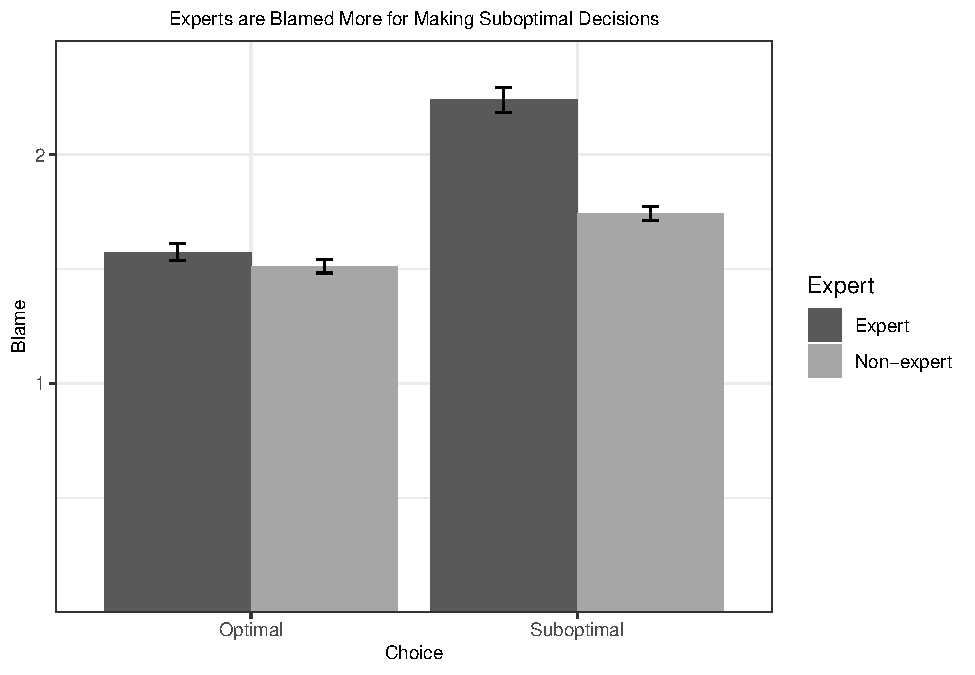
\includegraphics{ScientificReportManuscript_FINAL_files/figure-latex/fig-plot-1-1.pdf}
\caption{\label{fig:fig-plot-1}Mean ratings, based on choice, differ between experts and non-experts.}
\end{figure}

We next conducted analyses on each of the individual vignettes. These analyses included all participants who passed the comprehension check for the respective vignette, so the samples are larger than those reported in the main analyses above. For brevity, we report here only the key results, with full results presented in the Supplemental Materials. For the island vignette, the interactive effect of choice and expertise on blame was highly significant, \emph{F}(1, 770) = 10.62, \emph{p} = 0.001, \(n^2_p\) = 0.014. The optimality bias was present for experts, who were blamed more when they made the suboptimal choice (\emph{M} = 2.32, \emph{SD} = 1.88) as compared with the optimal choice (\emph{M} = 1.51, \emph{SD} = 1.17), \emph{F}(1, 770) = 31.00, \emph{p} \textless{} 0.001, \(n^2_p\) = 0.039; but it was not present for non-experts, for whom this difference was insignificant (\emph{M}\(_{50}\) = 1.81, \emph{SD} = 1.21 vs.~\emph{M}\(_{70}\) = 1.67, \emph{SD} = 1.33), \emph{F}(1, 770) = 0.997, \emph{p} = 0.32, \(n^2_p\) = 0.001).\\
For the ship vignette, the interaction of choice and expertise on blame was not significant, \emph{F}(1, 777) = 2.24, \emph{p} = 0.135, \(n^2_p\) = 0.003. Although this interaction was not significant, we once again observed that the optimality bias was present for experts (\emph{M}\(_{50}\) = 2.29, \emph{SD} = 1.78 vs.~\emph{M}\(_{70}\) = 1.80, \emph{SD} = 1.53), \emph{F}(1, 770) = 11.82, \emph{p} \textless{} 0.001, \(n^2_p\) = 0.015, but not for non-experts (\emph{M}\(_{50}\) = 1.80, \emph{SD} = 1.14 vs.~\emph{M}\(_{70}\) = 1.61, \emph{SD} = 1.10), \emph{F}(1, 770) = 1.84, \emph{p} = 0.175, \(n^2_p\) = 0.002.\\
Finally, we conducted several exploratory mediation analyses. For Studies 2, 3a, and 3b, we had originally preregistered running mediated moderation analyses of the overall interaction patterns. However, we later became convinced that these analyses were not as diagnostic as we had originally thought (see e.g., Edwards, 2009, pp. 156--157; Hayes, 2021, pp. 487--489). Accordingly, for each of these studies, we now report exploratory simple and parallel mediation models in only the condition in which we expected the optimality bias to occur (and not the experimental conditions in which we expected it to be diminished or eliminated). Although these analyses were not preregistered, their structure is identical across Studies 2, 3a, and 3b. We report the originally preregistered analyses in the Supplemental Materials.\\
For Study 2, we examined several simple and parallel mediation models in just the expert condition since this condition best captured the optimality bias. When both vignettes were combined, there was a significant indirect effect of negligence when entered as the sole mediator (a path = -0.81, \emph{p} \textless{} 0.001; b path = 0.66, \emph{p} \textless{} 0.001, ab path = -0.53, CI = -0.80 to -0.29; based on 5,000 bootstrap samples, Hayes PROCESS macro, Model 4), and a significant effect of need for explanation when it was entered alone (a path = 0.84, \emph{p} \textless{} 0.001; b path = -0.38, \emph{p} \textless{} 0.001, ab path = -0.34, CI = -0.64 to -0.04; based on 5,000 bootstrap samples, Model 4). When both mediators were entered together in a parallel mediation model, there was only a significant indirect effect of negligence (a path = -0.81, \emph{p} \textless{} 0.001; b path = 0.63, \emph{p} \textless{} 0.001, ab path = -0.51, CI = -0.77 to -0.28; based on 5,000 bootstrap samples, Model 4), and none for need for explanation (a path = -0.05, \emph{p} \textless{} 0.001; b path = -0.06, \emph{p} = 0.086, ab path = -0.05, CI = -0.12 to 0.01; based on 5,000 bootstrap samples, Model 4). Essentially the same pattern of results held when analyzing the island and ship vignettes individually, the only exception being that there were significant indirect effects of both negligence and need for explanation for the ship vignette (for full results, see the Supplemental Materials).

\hypertarget{discussion}{%
\section{Discussion}\label{discussion}}

Overall, the results of Study 2 support the mentalistic account of the optimality bias over the behaviorist account. Using two newly developed vignettes, we once again replicated the optimality bias, showing that individuals were blamed for making suboptimal choices, even though they apparently could not have known any better at the time of their choice. Critically, however, we found that this bias was significantly amplified among experts as compared with non-experts. The optimality bias (i.e., the blame difference for suboptimal vs.~optimal choices) was highly significant among experts, both when aggregating both vignettes together, and when analyzing each individually. But this effect was not significant among non-experts in the analysis that aggregated across vignettes, and not significant for either vignette when analyzed singularly. What explains this interaction? We surmise that the explanation fundamentally depends on mental state and capacity inferences. In essence, experts are believed to have a greater capacity to discern the correct path of action (even, apparently, when the lack of evidence renders that a formidable task), and as a consequence of these superior capacities, they are held to a higher epistemic standard than are non-experts. A purely behaviorist account, which explains optimality bias solely in terms of the relative efficiencies of optimal and suboptimal choices -- that is, the mere fact that a suboptimal choice is suboptimal -- cannot explain why the bias should be amplified for experts.\\
Mediation evidence tended to favor negligence over need for explanation, especially in joint mediation models, although both variables demonstrated significant indirect effects when analyzed in isolation. Study 3a was designed to provide another experimental means of testing the mentalist account of the optimality bias, and to provide further evidence on potential mediating processes.

\newpage

\hypertarget{references}{%
\section*{References}\label{references}}
\addcontentsline{toc}{section}{References}

\hypertarget{refs}{}
\begin{CSLReferences}{1}{0}
\leavevmode\vadjust pre{\hypertarget{ref-R-papaja}{}}%
Aust, F., \& Barth, M. (2022). \emph{{papaja}: {Prepare} reproducible {APA} journal articles with {R Markdown}}. Retrieved from \url{https://github.com/crsh/papaja}

\leavevmode\vadjust pre{\hypertarget{ref-baron1988a}{}}%
Baron, J., \& Hershey, J. C. (1988). Outcome bias in decision evaluation. \emph{Journal of Personality and Social Psychology}, \emph{54}(4), 569--579. \url{https://doi.org/10.1037/0022-3514.54.4.569}

\leavevmode\vadjust pre{\hypertarget{ref-R-tinylabels}{}}%
Barth, M. (2022). \emph{{tinylabels}: Lightweight variable labels}. Retrieved from \url{https://cran.r-project.org/package=tinylabels}

\leavevmode\vadjust pre{\hypertarget{ref-birch2007a}{}}%
Birch, S. A., \& Bloom, P. (2007). The curse of knowledge in reasoning about false beliefs. \emph{Psychological Science}, \emph{18}(5), 382--386. \url{https://doi.org/10.1111/j.1467-9280.2007.01909.x}

\leavevmode\vadjust pre{\hypertarget{ref-birch2017a}{}}%
Birch, S. A., Brosseau-Liard, P. E., Haddock, T., \& Ghrear, S. E. (2017). A {``curse of knowledge''} in the absence of knowledge? People misattribute fluency when judging how common knowledge is among their peers. \emph{Cognition}, \emph{166}, 447--458. \url{https://doi.org/10.1016/j.cognition.2017.04.015}

\leavevmode\vadjust pre{\hypertarget{ref-cusimano2020a}{}}%
Cusimano, C., \& Goodwin, G. P. (2020). People judge others to have more voluntary control over beliefs than they themselves do. \emph{Journal of Personality and Social Psychology}, \emph{119}(5), 999--1029. \url{https://doi.org/10.1037/pspa0000198}

\leavevmode\vadjust pre{\hypertarget{ref-dennett1987a}{}}%
Dennett, D. C. (1987). \emph{The intentional stance}. Cambridge, Massachusetts: MIT Press.

\leavevmode\vadjust pre{\hypertarget{ref-disease2021a}{}}%
Disease Control, C., \& Prevention. (2021). \emph{Previous u.s. COVID-19 case data}. Retrieved from \url{https://covid.cdc.gov/covid-data-tracker/\#datatracker-home.}

\leavevmode\vadjust pre{\hypertarget{ref-edwards2009a}{}}%
Edwards, J. R. (2009). \emph{Seven deadly myths of testing moderation in organizational}.

\leavevmode\vadjust pre{\hypertarget{ref-fischhoff2007a}{}}%
Fischhoff, B. (2007). An early history of hindsight research. \emph{Social Cognition}, \emph{25}(1), 10--13. \url{https://doi.org/10.1521/soco.2007.25.1.10}

\leavevmode\vadjust pre{\hypertarget{ref-freitas2018a}{}}%
Freitas, J., \& Johnson, S. G. (2018). Optimality bias in moral judgment. \emph{Journal of Experimental Social Psychology}, \emph{79}, 149--163. \url{https://doi.org/10.1016/j.jesp.2018.07.011}

\leavevmode\vadjust pre{\hypertarget{ref-fumento2020a}{}}%
Fumento, M. (2020). Erosion of trust: 10 things public health establishment got wrong about coronavirus. \emph{Just the News}. Retrieved from \url{https://justthenews.com/politics-policy/coronavirus/erosion-trust-10-things-public-health-establishment-got-wrong-about}

\leavevmode\vadjust pre{\hypertarget{ref-gerace2015a}{}}%
Gerace, A., Day, A., Casey, S., \& Mohr, P. (2015). Perspective taking and empathy: Does having similar past experience to another person make it easier to take their perspective? \emph{Journal of Relationships Research}, \emph{6}(10), 1--14. \url{https://doi.org/10.1017/jrr.2015.6}

\leavevmode\vadjust pre{\hypertarget{ref-gergely2013natural}{}}%
Gergely, G., \& Csibra, G. (2013). Natural pedagogy. \emph{Navigating the Social World: What Infants, Children, and Other Species Can Teach Us}, 127--132.

\leavevmode\vadjust pre{\hypertarget{ref-greenhut2020a}{}}%
Greenhut, S. (2020). \emph{Shocker! The experts were wrong. R street}. Retrieved from \url{https://www.rstreet.org/2020/06/04/shocker-the-experts-were-wrong/}

\leavevmode\vadjust pre{\hypertarget{ref-hayes2021a}{}}%
Hayes, A. F. (2021). \emph{Introduction to mediation, moderation, and conditional process analysis}. Guilford Press.

\leavevmode\vadjust pre{\hypertarget{ref-isler2020a}{}}%
Isler, O., Yilmaz, O., \& Dogruyol, B. (2020). Activating reflective thinking with decision justification and debiasing training. \emph{Judgment and Decision Making}, \emph{15}(6), 926--938. Retrieved from \url{http://journal.sjdm.org/20/201008/jdm201008.html}

\leavevmode\vadjust pre{\hypertarget{ref-johnson2015a}{}}%
Johnson, S. G., \& Rips, L. J. (2015). Do the right thing: The assumption of optimality in lay decision theory and causal judgment. \emph{Cognitive Psychology}, \emph{77}, 42--76. \url{https://doi.org/10.1016/j.cogpsych.2015.01.003}

\leavevmode\vadjust pre{\hypertarget{ref-kulldorff2021a}{}}%
Kulldorff, M., \& Bhattacharya, J. (2021). \emph{How fauci fooled america}. Newsweek. Retrieved from \url{https://www.rstreet.org/2020/06/04/shocker-the-experts-were-wrong/}

\leavevmode\vadjust pre{\hypertarget{ref-lance-a}{}}%
Lance, C. E., \& Vanderberg, R. J. (Eds.). (n.d.). Research. In \emph{Statistical and methodological}.

\leavevmode\vadjust pre{\hypertarget{ref-leape2000a}{}}%
Leape, L. L., \& Berwick, D. M. (2000). Medical error: The second victim. \emph{BMJ}, \emph{320}, 785--788.

\leavevmode\vadjust pre{\hypertarget{ref-malle2021moral}{}}%
Malle, B. F. (2021). Moral judgments. \emph{Annual Review of Psychology}, \emph{72}, 293--318.

\leavevmode\vadjust pre{\hypertarget{ref-malle2014theory}{}}%
Malle, B. F., Guglielmo, S., \& Monroe, A. E. (2014). A theory of blame. \emph{Psychological Inquiry}, \emph{25}(2), 147--186.

\leavevmode\vadjust pre{\hypertarget{ref-martin2016a}{}}%
Martin, J. W., \& Cushman, F. (2016). The adaptive logic of moral luck. In J. Sytsma \& W. Buckwalter (Eds.), \emph{A companion to experimental philosophy} (pp. 190--202). John Wiley \& Sons, Ltd.

\leavevmode\vadjust pre{\hypertarget{ref-R-Require}{}}%
McIntire, E. J. B. (2023). \emph{Require: Installing and loading r packages for reproducible workflows}. Retrieved from \url{https://CRAN.R-project.org/package=Require}

\leavevmode\vadjust pre{\hypertarget{ref-newman2018a}{}}%
Newman, L. S., Tan, M., Caldwell, T. L., Duff, K. J., \& Winer, E. S. (2018). Name norms: A guide to casting your next experiment. \emph{Personality and Social Psychology Bulletin}, \emph{44}(10), 1435--1448. \url{https://doi.org/10.1177/0146167218769858}

\leavevmode\vadjust pre{\hypertarget{ref-pappas2012a}{}}%
Pappas, S. (2012). \emph{Italian scientists sentenced to 6 years for earthquake statements}. Scientific American. Retrieved from \url{https://www.scientificamerican.com/article/italian-scientists-get/}

\leavevmode\vadjust pre{\hypertarget{ref-R-base}{}}%
R Core Team. (2021). \emph{R: A language and environment for statistical computing}. Vienna, Austria: R Foundation for Statistical Computing. Retrieved from \url{https://www.R-project.org/}

\leavevmode\vadjust pre{\hypertarget{ref-ross1977a}{}}%
Ross, L. (1977). The intuitive psychologist and his shortcomings: Distortions in the attribution process. In \emph{Advances in experimental social psychology} (Vol. 10, pp. 173--220). Academic Press. \url{https://doi.org/10.1016/S0065-2601(08)60357-3}

\leavevmode\vadjust pre{\hypertarget{ref-royzman2015a}{}}%
Royzman, E. B., Kim, K., \& Leeman, R. F. (2015). The curious tale of julie and mark: Unraveling the moral dumbfounding effect. \emph{Judgment and Decision Making}, \emph{10}(4).

\leavevmode\vadjust pre{\hypertarget{ref-spellman2014a}{}}%
Spellman, B. A., \& Gilbert, E. A. (2014). Blame, cause, and counterfactuals: The inextricable link. \emph{Psychological Inquiry}, \emph{25}(2), 245--250. \url{https://doi.org/10.1080/1047840X.2014.901708}

\leavevmode\vadjust pre{\hypertarget{ref-spellman2001a}{}}%
Spellman, B. A., \& Kincannon, A. (2001). The relation between counterfactual ({``but for''}) and causal reasoning: Experimental findings and implications for jurors' decisions. \emph{Law and Contemporary Problems}, \emph{64}(4), 241--264. \url{https://doi.org/10.2307/1192297}

\end{CSLReferences}


\end{document}
